\section{Actors and use-cases}
\label{sec:use-case}

In this section we define the actors who will use our method to collaborate.
Then we present the use-cases of a generic development environment used by
the actors. The use-cases are the functionalities that the development environment
must have for model-code synchronization.

\subsection{Actors}

In this paper we propose a method for collaboration between model-driven developers
and code-driven developers, who are thus the actors who will use the proposed method.
Before defining these actors, let us first define the concept of development artifact and reference artifact.

% TODO find standard definition
\begin{definition}[Development artifact]
A development resource is a resource that contains enough information
for the implementation of the system.
\end{definition}

For example a system can be entirely implemented as code.
The code project is then a development artifact.
A model may also be a development artifact.
It is then not only documentation of specification.
For example a model can be used for implementation either by compiling
it directly \cite{asma}, or by generating code from the model, and compiling the code without
the need to modify it.

% TODO find standard definition
\begin{definition}[Reference artifact]
A reference artifact is one which may be modified manually.
All other artifacts are produced from the reference artifact
through some process, and only through the process. Manual modification
of artifacts other than the reference artifact is forbidden.
\end{definition}

The actors who will use our method are called 
model-driven developer and code-driven developers.
Both are developers which is defined as follows:

\begin{definition}[Developer \cite{developer_def_ref}]
TODO: find a definition in standard docu
\end{definition}

The main difference between a model-driven developer and a code-driven developer
is what they consider as the reference artifact.

% TODO find standard definition
\begin{definition}[Model-driven developer]
A model-driven developer is a developer for whom the model is the reference artifact
during development.
\end{definition}

Otherwise said, for the model-driven developer only the model should be modified manually. The
code must always be produced from the model through some process that guarantees that the
code is conform to the model. Note that in the case of an object-oriented model, not only
is the architecture of the project stored in the model, but also the implementation of
methods.

% TODO find standard definition
\begin{definition}[Code-driven developer]
A model-driven developer is a developer for whom the code is the reference artifact
during development.
\end{definition}

\subsection{Use-cases}

In this section we propose a development environment with
use-cases that make it possible for the actors to develop
the system with their development preferences.
Figure \ref{fig:use-case} shows a UML use-case diagram of the development environment
and their associations to the actors. (UML notations are used.)

% TODO: bold text in figure
\begin{figure}
\centering
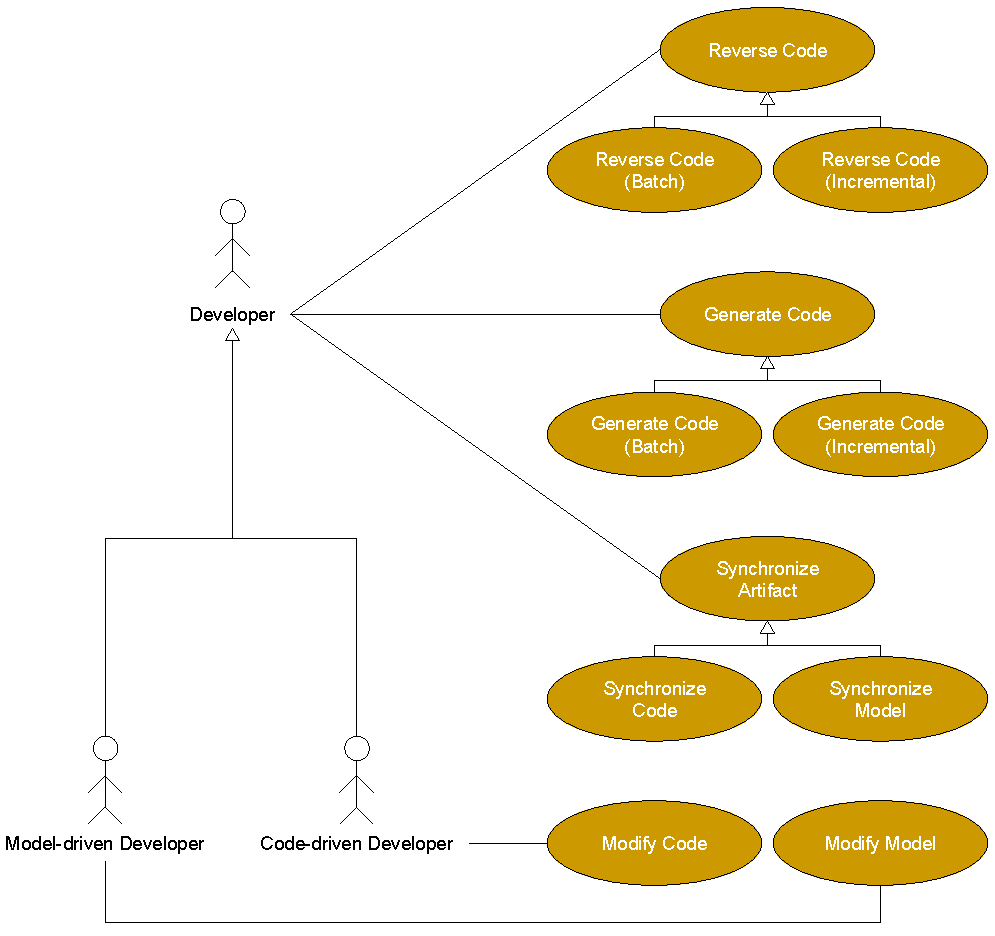
\includegraphics[width=\columnwidth]{figures/use-case}
\caption{Use-case Diagram} 
\label{fig:use-case}
\end{figure}

There are some use-cases for manual modification of artifacts. The \textbf{Modify Artifact} use-case
means the development environment must have some tool to let the developer manually modify an artifact.
The \textbf{Modify Model} and \textbf{Modify Code} use-cases are specializations of the \textbf{Modify Artifact}
use-case where model and code are respectively the artifact in question.

There are also some use-case for the synchronization of artifacts. The \textbf{Synchronize Artifact} use-case
is the synchronization of two artifacts by updating each artifact to reflect changes made to the other artifact,
and by reconciling conflicts between the artifacts. The \textbf{Synchronize Model} and \textbf{Synchronize Code}
use-cases are specializations where model and code are respectively the artifact in question.

Finally there are some use-cases for producing one artifact from the other and vice versa.
The \textbf{Generate Code} use-case is the production of code in a programming language from a model in a modeling language.
This use-case is related to forward engineering \cite{forward_engineering_ref} which is the production
of implementation from specification.
% Do we need this definition of forward engineering? Isn't it more confusion actually since we 'implementation' and 'specification' keywords.
The developer can either use \textbf{Generation Code (Batch)} or \textbf{Generate Code (Incremental)}. Batch
code generation produces new code from the model. If any code existed before, it is overwritten entirely with
the new code. Incremental code generation is [Official definition here].

The \textbf{Reverse Code} use-case is the production of model in a modeling language from code in a programming language.
This use-case is related to \cite{reverse_engineering_ref} which is the production of specification from implementation.
% Do we need this definition of reverse engineering? Same reasons as above.
The developer can either use \textbf{Reverse Code (Batch)} or \textbf{Reverse Code (Incremental)}.
Like their counter-part in the code generation use-cases, the difference between batch and
incremental reverse is the how the produced artifact is updated or overwritten.
